\section{Onde}

\subsection{Caratterizzazione delle onde}
\begin{itemize}
    \item Onde meccaniche(possono esistere solo in un mezzo materiale)
    \item onde elettromeccaniche(possono esistere nel vuoto)
\end{itemize}

Per le onde meccaniche, si devono distinguere due aspetti:
\begin{itemize}
    \item moto(propagazione) dell'onda attraverso il mezzo
    \item moto della particella del mezzo materiale
\end{itemize}

\begin{figure}[H]
    \centering
    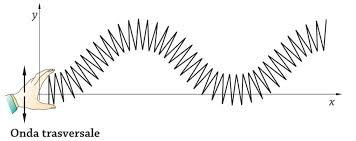
\includegraphics[width=0.45\linewidth]{imgs/22 - onda 2.png}
    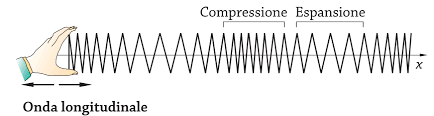
\includegraphics[width=0.45\linewidth]{imgs/21 - onde.png}
    \label{fig:onda}
    \caption{Esempio di onde in due movimenti}
\end{figure}

\subsection{Onda piana}
Una funzione d'onda è composta di $f(\vec{r},t)$ dove r è la posizione
e t il tempo.
Un'onda pina dipende solo da una direzione.



\subsection{Onde armoniche}
\begin{equation}
    f(x \pm vt) = A\sin(kx \pm \omega t + \phi)
\end{equation}

\begin{itemize}
    \item $A$ è l'ampiezza dell'onda
    \item $kx \pm \omega t + \phi$ è la fase
    \item $k$ è il numero d'onda(rad/m)
    \item $\omega$ è la pulsazione(freq angolare(rad/s))
    \item $\phi$ è la fase iniziale
\end{itemize}

Ricordati che puoi ottenere la frequenza usando $f = \frac{\omega}{2\pi}$.

L'onda armonica è progressiva/regressiva se:
\begin{equation}
    \frac{\omega}{k} = v
\end{equation}

Per l'onda progressiva, la funzione è periodica al tempo:
\begin{equation}
    T = \frac{2\pi}{\omega}
\end{equation}
e rispetto alle coordinate spaziali(lunghezza d'onda):
\begin{equation}
    \lambda = \frac{2\pi}{k}
\end{equation}

Ovviamente la velocità di propagazione sarà spazio fratto tempo:
\begin{equation}
    \frac{\lambda}{T} = \frac{\omega}{k} = v
\end{equation}

\subsection{Energia, potenza, intensità di un'onda}

La potenza si trova facendo:
\begin{equation}
    P = \frac{\Delta E}{\Delta t} = u^{(lin)}v
\end{equation}

